\documentclass[ignorenonframetext]{beamer}
\mode<article>
{
\usepackage{fullpage}
}

\mode<presentation>
{
  \usetheme{Boadilla}
  \setbeamertemplate{navigation symbols}{}
  \usefonttheme[onlymath]{serif}
}

\usepackage[english]{babel}
% or whatever
\usepackage{pgf}
\usepackage{tikz}
\usepackage{amsmath}
\usepackage{amsfonts}
\usepackage{multimedia}
\usepackage[latin1]{inputenc}
\usepackage{xmpmulti}
\usepackage{times}
\usepackage[T1]{fontenc}
% Or whatever. Note that the encoding and the font should match. If T1
% does not look nice, try deleting the line with the fontenc.
\usepackage{multimedia}
\usepackage{hyperref}

\usetikzlibrary{shapes,arrows}

%\input{Templates/math_macros.tex}

\newcommand{\degree}{\ensuremath{^\circ}}

\title[] % (optional, use only with long paper titles)
{Mining Flickr}

\subtitle
{} % (optional)

\author[AE-AJW]% (optional, use only with lots of authors)
{Armin Eftekhari \\ Alejandro Weinstein}
% - Use the \inst{?} command only if the authors have different
%   affiliation.

\institute[CSM] % (optional, but mostly needed)
{Division of Engineering\\
  Colorado School of Mines}
% - Use the \inst command only if there are several affiliations.
% - Keep it simple, no one is interested in your street address.

\date {December 7, 2009}% (optional)


% If you have a file called "university-logo-filename.xxx", where xxx
% is a graphic format that can be processed by latex or pdflatex,
% resp., then you can add a logo as follows:

%\pgfdeclareimage[height=1.1cm]{university-logo}{UniversityLogo}
%\logo{\pgfuseimage{university-logo}}

\begin{document}
% For every picture that defines or uses external nodes, you'll have to
% apply the 'remember picture' style. To avoid some typing, we'll apply
% the style to all pictures.


% By default all math in TikZ nodes are set in inline mode. Change this to
% displaystyle so that we don't get small fractions.
\everymath{\displaystyle}
\begin{frame}
  \titlepage
\end{frame}

\section{Introduction}

\begin{frame}{Key idea}
Is there any relationship between the popularity of a photo and the camera used?
\begin{center}
\includegraphics[scale=0.25]{most_popular.jpg}
\begin{center}
\tiny{\url{http://www.flickr.com/photos/acastellano/181730235/}}
\end{center}
\end{center}
\begin{itemize}
\item 2573 comments
\item 69 tags
\item 8539 users call this photo a favorite
\item Taken with a Canon EOS 10D (about \$1000).
\end{itemize}
\end{frame}

\begin{frame}{Key idea}
\begin{center}
\includegraphics[scale=0.35]{not_popular.jpg}
\begin{center}
\tiny{\url{http://www.flickr.com/photos/luigistrano/354904253}}
\end{center}
\end{center}
\begin{itemize}
\item 17 comments
\item 15 tags
\item 7 users call this photo a favorite
\item Taken with a Panasonic DMC-FX7 (about \$400).
\end{itemize}
\end{frame}

\begin{frame}{Building the data set}
Build using the Flickr API, using the Python ``Flickr API kit''. We get the following attributes:

\begin{description}
\item[Id:] the unique id used by Flickr to identify a photo.
\item[Views:] the number of views of the photo.
\item[Location:] the location of the photo.
\item[Comments:] the number of comments of the photo.
\item[Tags:] the number of tags of the photo.
\item[Favorites:] the number of Flickr users that call the photo a favorite
\item[Make:] the maker of the camera used to take the photo.
\item[Model:] the model of the camera used to take the photo.
\end{description}
\end{frame}

\begin{frame}{Building the data set}
Sampling strategy: 
\begin{itemize}
\item Get 100 photos for each of the ``All time most popular tags''.
\item The photos must be at least one year old.
\item Four steps process:
\begin{enumerate}
\item Get the 100 ids for each of the poplular tags. We got 14400 records.
\item Eliminate the duplicate ids. We reduced the 14400 records to 7342.
\item Get the data for each photo id.
\item Write the data as a CSV file.
\end{enumerate}
\end{itemize}

Building the dataset took several hours.
\end{frame}

\begin{frame}{Dataset cleaning}
\begin{itemize}
\item The \emph{Make} attribute was inconsistent.
\item Slightly different names for a given maker. 
\item For instance, ``Olympus'' cameras were labeled as ``Olympus Imaging Corp.'', ``Olympus optical Co. Ltd'' or ``Olympus corporation''. 
\item Another Python script  solved this inconsistency.
\item We reduced the number of unique manufacturers from 62 to 36.
\end{itemize}
\end{frame}

\begin{frame}{Summary statistics: Favorites}
\begin{center}
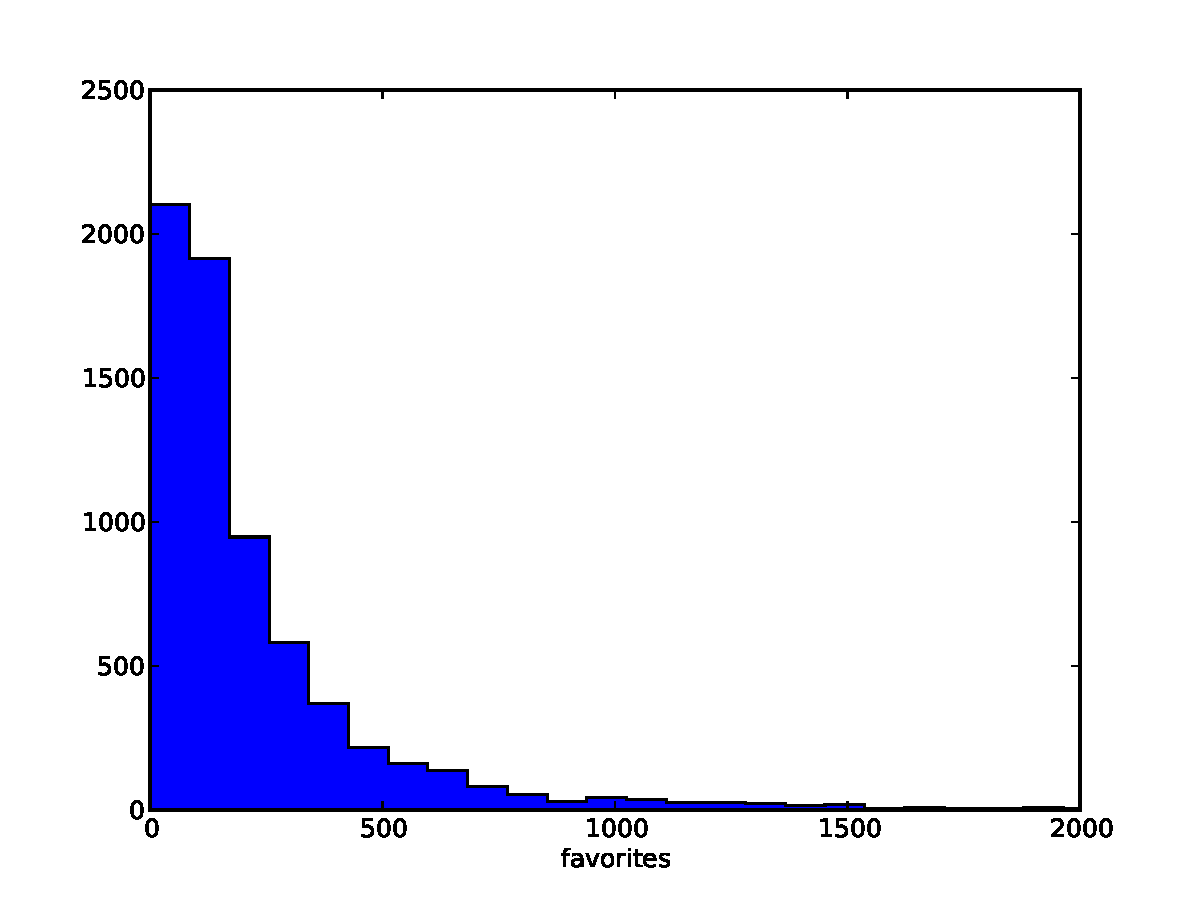
\includegraphics[scale=0.35]{histo_favorites.pdf}
\end{center}
\begin{center}
\begin{tabular}{|l|l|}
\hline\multicolumn{2}{|c|}{favorites} \\
\hline
Min & 0 \\
Max & 8539 \\
Mean & 243.0\\
Std dev & 348.2 \\
\hline
\end{tabular}
\end{center}
\end{frame}

\begin{frame}{Summary statistics: Makers}
\begin{center}
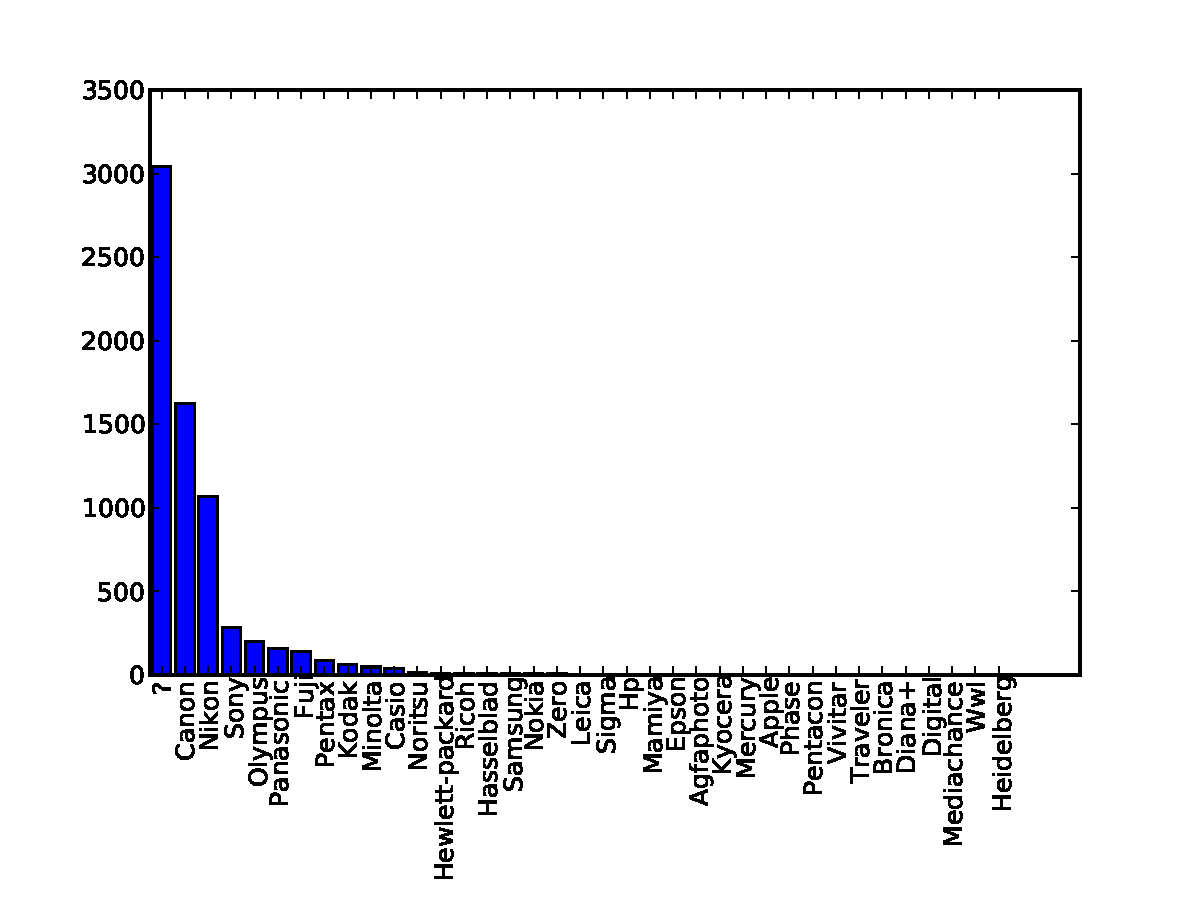
\includegraphics[scale=0.5]{histo_make.pdf}
\end{center}
\end{frame}

\begin{frame}{Scatter plot}
\begin{center}
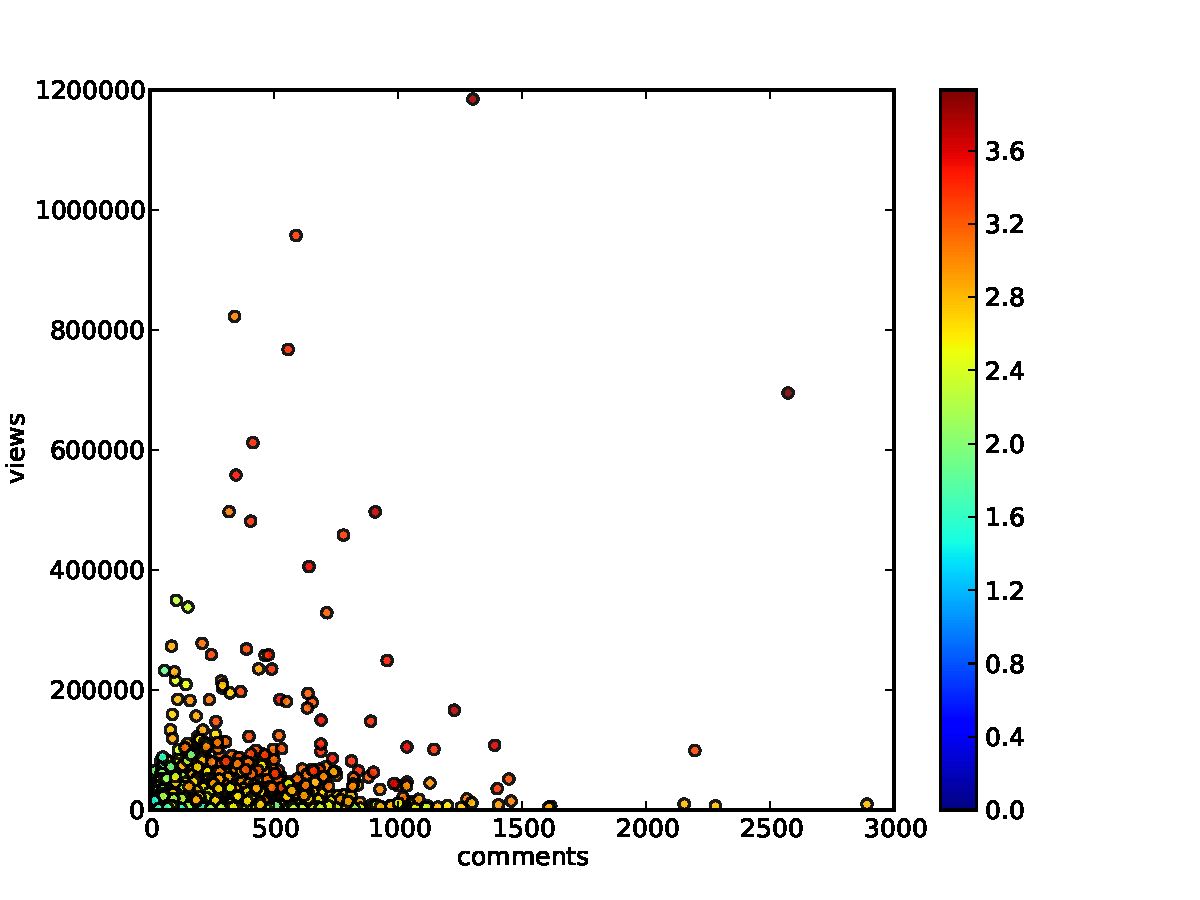
\includegraphics[scale=0.5]{scatter.pdf}
\end{center}
\end{frame}


\begin{frame}[fragile]{Clustering}
\begin{verbatim}
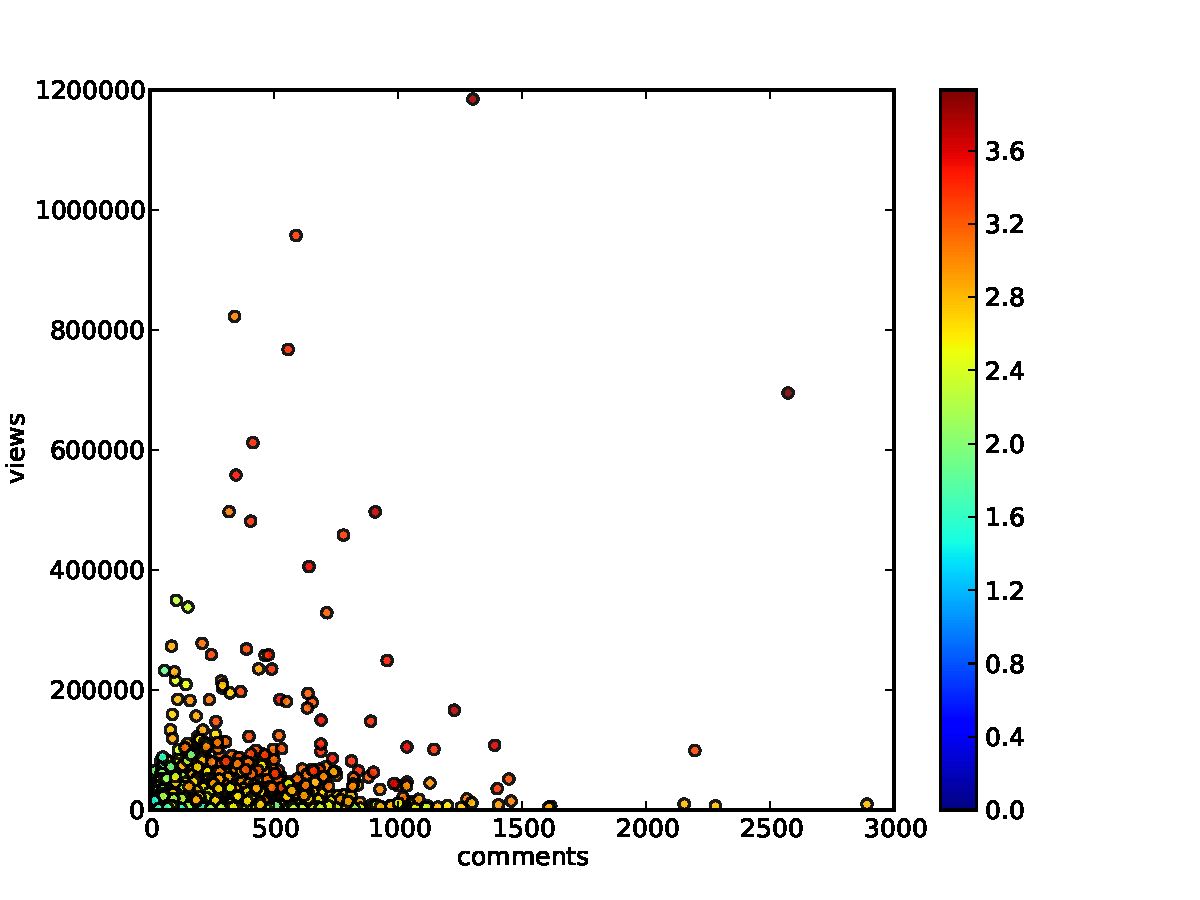
\includegraphics[scale=0.5]{scatter.pdf}
\end{verbatim}
\end{frame}
     

\begin{frame}{Clustering}
\begin{center}
\includegraphics[scale=0.5]{favorites-comments.png}
\end{center}
\end{frame}

\begin{frame}{Clustering}
\begin{center}
\includegraphics[scale=0.5]{model_favor.png}
\end{center}
\end{frame}

\begin{frame}{Clustering}
\begin{center}
\includegraphics[scale=0.5]{view_comments.png}
\end{center}
\end{frame}

\end{document}
